\section{Exercise VII: Support Vector Machines}

\bullet \  We write the corresponding Kernel function associated to $\Phi$.\\ \\
$\forall \textbf{x} = (x_1, x_2) \in \mathbb{R}^2, \forall \mathbf{y} = (y_1, y_2) \in \mathbb{R}^2:$
\begin{align*}
    K\left(\mathbf{x}, \mathbf{y} \right) 
    &= \langle \Phi(x_1, x_2), \Phi(y_1, y_2) \rangle \\
    &= 2x_1y_1 + 2x_1x_2y_1y_2 + 1 + 2x_2y_2 + x_1^2y_1^2 + x_2^2y_2^2 \\
    &= (x_1y_1 + x_2y_2 + 1)^2 \\
    &\boxed{= (\mathbf{x}^T \mathbf{y} + 1)^2.}
\end{align*}

This a polynomial Kernel of order 2 that is convex and differentiable.\\ \\
\bullet \ Let's try to give the expression of the corresponding SVM solution. We define: 
\[
\mathbf{x}^1 = (1, 1); \quad
\mathbf{x}^2 = (-1, _1); \quad
\mathbf{x}^3 = (1, -1); \quad
\mathbf{x}^4 = (-1, 1); \quad
y^1 = 1; \quad
y^2 = 1; \quad
y^3 = -1; 
\]
\[
y^4 = -1;\quad
\mathbf{w} = \sum_{i=1}^{4} \alpha_i y^i \Phi(\mathbf{x}^i) \text{ with } (\alpha_i)_{1 \le i \le 4} \in \mathbb{R}^4.
\]
We now want to find the optimal $(\alpha_i^{*})_{1 \le i \le 4}$ that minimize the following function:
\[
    \mathcal{L}(\mathbf{w}, b, \alpha)=\sum_{i=1}^n \alpha_i-\frac{1}{2} \sum_{i, j=1}^n \alpha_i \alpha_j y^i y^j K\left(x^i, x^j\right), \\
\]
with the condition,
\[
    \sum_{i=1}^n \alpha_i y^i = \alpha_1 + \alpha_2 - \alpha_3 - \alpha_4 = 0.
\]
With observe that:
\[
    \forall i \in \llbracket 1, 4 \rrbracket, \quad K(\mathbf{x^i}, \mathbf{x^i}) = 9 ; \quad
    \forall (i, j) \in \llbracket 1, 4 \rrbracket^2, \text{ s.t. } i \neq j, \quad K(\mathbf{x^i}, \mathbf{x^i}) = 1.
\]
By direct calculus,
\[
    \mathcal{L}(\mathbf{w}, b, \alpha) = \alpha_1 + \alpha_2 + \alpha_3 + \alpha_4 - \alpha_1 \alpha_2 - \alpha_3 \alpha_4 + \alpha_1 \alpha_3 +\alpha_1 \alpha_4 + \alpha_2 \alpha_3 + \alpha_2 \alpha_4 \\
    -\frac{1}{2}\alpha_1^2 -\frac{1}{2}\alpha_2^2 -\frac{1}{2}\alpha_3^2 -\frac{1}{2}\alpha_4^2.
\]
By using the condition on alphas:
\[
    \frac{\partial \mathcal{L}}{\partial \alpha_1} (\mathbf{w}, b, \alpha) = 1 - \alpha_2 + \alpha_3 + \alpha_4 - 9\alpha_1 = 1 - 8\alpha_1;
\]
\[
    \frac{\partial \mathcal{L}}{\partial \alpha_2} (\mathbf{w}, b, \alpha) = 1 - \alpha_1 + \alpha_3 + \alpha_4 - 9\alpha_2 = 1 - 8\alpha_2;
\]
\[
    \frac{\partial \mathcal{L}}{\partial \alpha_3} (\mathbf{w}, b, \alpha) = 1 - \alpha_4 + \alpha_1 + \alpha_2 - 9\alpha_3 = 1 - 8\alpha_3;
\]
\[
    \frac{\partial \mathcal{L}}{\partial \alpha_4} (\mathbf{w}, b, \alpha) = 1 - \alpha_3 + \alpha_1 + \alpha_2 - 9\alpha_4 = 1 - 8\alpha_4.
\]
This means that, by cancelling the partial derivatives,

\[
    \boxed{
    \forall i \in \llbracket 1 , 4 \rrbracket, \quad
    \alpha_i^* = \frac{1}{8}.
    }
\]
Since $K$ is a convex differentiable function, any point where the gradient is 0 is a minimum; so this indeed the minimum of $\mathcal{L}$.\\ \\
After,
\[
    \boxed{
    \mathbf{w^*} = \frac{1}{8}(\Phi(\mathbf{x^1}) + \Phi(\mathbf{x^2}) - \Phi(\mathbf{x^3}) - \Phi(\mathbf{x^4})) = \frac{1}{2}
    \begin{pmatrix}
        0 \\
        \sqrt{2} \\
        0 \\
        0 \\
        0 \\
        0
    \end{pmatrix}.
    }
\]

\bullet \ Then,

\[
    \boxed{
    b^*=-\frac{\max _{i: y^i=-1}\left\langle\mathbf{w}^*, \mathbf{x}^i\right\rangle+\min _{i: y^i=+1}\left\langle\mathbf{w}^*, \mathbf{x}^i\right\rangle}{2} = 0.
    }
\]
Thus, the equation of the separating hyperplane for $\mathbf{x} \in \mathbb{R}^6$ is:
\[
    \mathbf{w}^T\mathbf{x} + b^* = 0 \Longleftrightarrow \boxed{x_2 = 0.}
\]
The two hyperplane through the support vectors are given by the equation $\mathbf{w}^T\mathbf{x} + b^* = \pm 1$, which give:
\[
    \boxed{x_2 = \sqrt{2} \text{ and } x_2 = -\sqrt{2}.}
\]

\begin{figure}
    \centering
    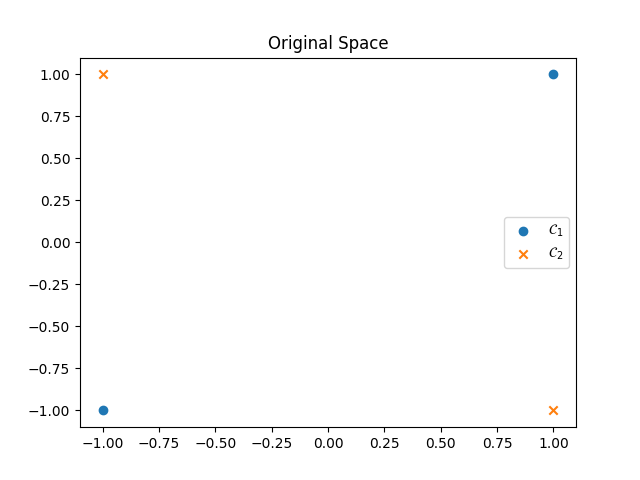
\includegraphics[width=0.65\textwidth]{exercise6_assets/original_space.png}
    \caption{The plot on the original space.}
    \label{fig:original-space}
\end{figure}

\begin{figure}
    \centering
    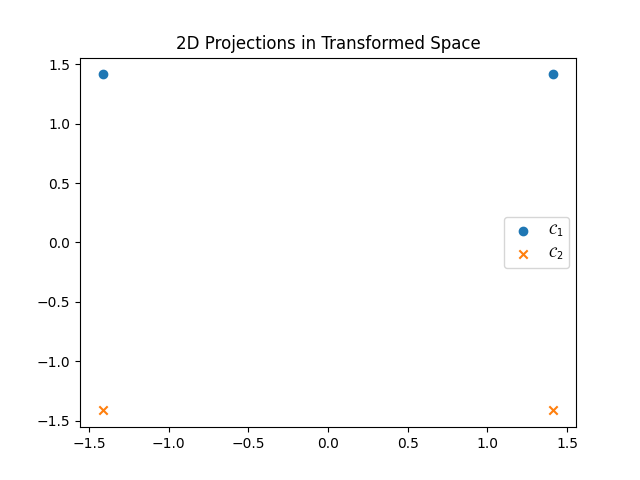
\includegraphics[width=0.65\textwidth]{exercise6_assets/transformed_space.png}
    \caption{The plot of the 2D projections onto the transformed space.}
    \label{fig:transformed-space}
\end{figure}